\section{Architettura del sistema}
L'applicazione ADCrm presenta un'architettura client-server, assumendo entrambi i ruoli:
\paragraph{Server}
L'applicazione assume il ruolo di server nel momento in cui deve assolvere alle richieste che arrivano da ADProject mediante le API REST. Deve quindi rispondere ad un'esigenza principale due esigenze:
\begin{itemize}
	\item esporre API REST per poter rispondere, in formato \glo{JSON}, alle richieste HTTP ricevute;
	\item salvare le credenziali per il processo di autenticazione e collegamento con il CRM su un piccolo database interno.
\end{itemize} 

Si è deciso di mantenere il database sul servizio ADCrm per togliere l'onere ad ADProject di conoscere: non solo le procedure di autenticazione al CRM, ma anche la tipologia di CRM che si va ad interrogare (Salesforce, Dynamics, ...). In questo modo si riesce a mantenere una netta separazione dei ruoli tra le varie componenti. 

\paragraph{Client}
L'applicazione funge da client nel momento in cui deve interrogare il server del CRM per recuperare i dati di cui ha bisogno ADProject; deve quindi:
\begin{itemize}
	\item interrogare il server remoto attraverso il set di API che espone;
	\item organizzare i dati ricevuti in modo tale che siano fruibili da ADProject.
\end{itemize}

Nelle prime fasi della progettazione si è valutata l'ipotesi di utilizzare un database per fare \glo{caching} dei dati provenienti dal CRM, così da limitare le richieste HTTP necessarie e da velocizzare le risposte fornite, tuttavia la necessità di ADProject di utilizzare sempre dati aggiornati ha fatto abbandonare quest'opzione.\\

La figura \ref{fig:architetturasistema} illustra l'architettura ad alto livello del sistema; una descrizione più dettagliata delle varie componenti verrà esposta nelle sezioni successive.

\begin{figure}[H]
	\centering
	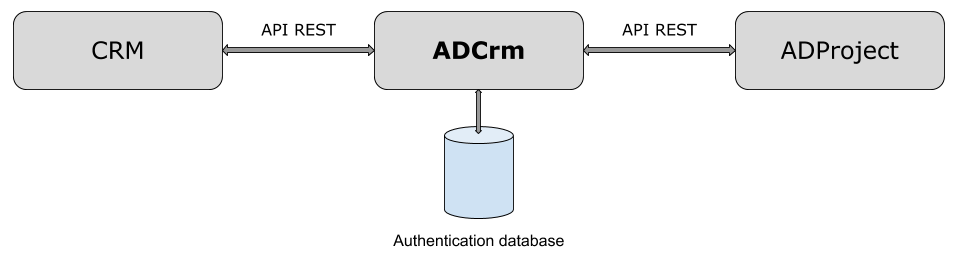
\includegraphics[width=\linewidth]{images/architettura_sistema}
	\caption{Architettura ad alto livello}
	\label{fig:architetturasistema}
\end{figure}

\section{API REST}
Di seguito si trova la definizione delle API REST esposte dal servizio ADCrm.\\
I metodi HTTP con cui chiamare tutti i successivi URL sono metodi \textbf{GET} ed i dati ricevuti nelle risposte sono forniti in formato \glo{JSON}.

	\begin{small}
		\begin{longtable}{ | l | p{8cm} | }
			\hline \textbf{URL} & \textbf{Descrizione Risposta}\\
			\hline api/organization/\{organizationId\}/ & Risponde con i dati riguardante l'organizzazione avente id = \{organizationId\}\\
			\hline
		\end{longtable}		
	\end{small}
Questo primo \glo{endpoint} necessita di ulteriori spiegazioni in quanto l'url specificato sopra è da anteporre a di tutti quelli che seguiranno (eg. "\textbf{api/organization/\{organizationId\}/accounts}" nel caso dell'url "/accounts").\\
Inoltre si noti che è necessario da parte di chi effettua chiamate verso questo url (e quindi anche verso tutti gli altri) conoscere il campo \{organizationId\} per poter ottenere una risposta. Questa restrizione è stata posta per far si che il sistema sia più sicuro, rendendo disponibili dei dati riguardanti l'azienda fruitrice del servizio solo se si conosce il corretto identificativo.
%TODO: decidere se sistemare la parte qua sopra
	\begin{small}
		\begin{longtable}{ | l | p{8cm} | }
			\hline \textbf{URL} & \textbf{Descrizione Risposta}\\
			\hline /accounts & Risponde con la lista contenente i dati di tutti gli account\\
			\hline /accounts/\{\textit{accountId}\} & Risponde con i dati dell'account avente \textit{id = accountId}\\    
			\hline /accounts/\{\textit{accountId}\}/contacts & Risponde con la lista contenente i dati di tutti gli i contatti legati all'account avente \textit{id = accountId}\\
			\hline /contacts/\{\textit{contactId}\} & Risponde con i dati del contatto avente \textit{id = contactId}\\
			\hline /proposals & Risponde con la lista contenente i dati di tutte le proposte commerciali\\
			\hline /proposals/\{\textit{proposalId}\} & Risponde con i dati della proposta commerciale avente \textit{id = proposalId}\\    
			\hline /proposals/\{\textit{proposalId}\}/products & Risponde con una lista contenente tutti i prodotti legati all'offerta commerciale avente \textit{id =  proposalId}\\
			\hline /products/\{\textit{productId}\} & Risponde con i dati del prodotto avente \textit{id = productId}\\
			\hline /users & Risponde con una lista contenente i dati di tutti gli utenti del CRM\\
			\hline /users/\{\textit{userId}\} & Risponde con i dati del utente avente \textit{id = userId}\\    
			\hline /productCategories & Risponde con una lista contenente i dati di tutte le famiglie di prodotti\\
			\hline /productCategories/\{\textit{categoryId}\} & Risponde con i dati della famiglia di prodotti avente \textit{id = categoryId}\\		
			\hline 
		\end{longtable}		
	\end{small}
	
\section{Progettazione di dettaglio}

\begin{figure}[H]
	\centering
	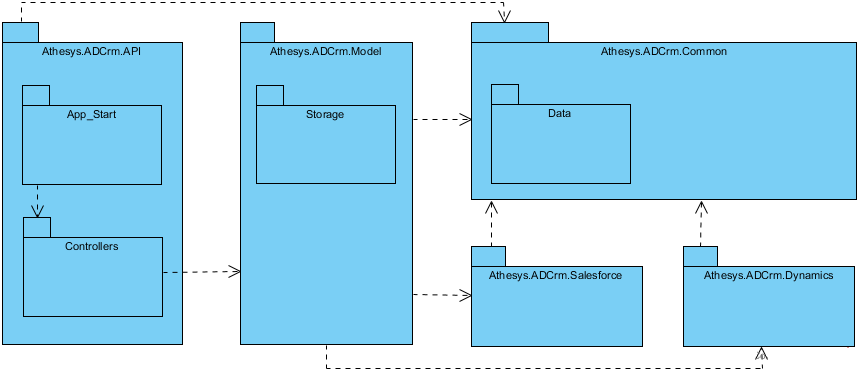
\includegraphics[width=\linewidth]{images/modulesDiagram}
	\caption{Diagramma dei moduli di ADCrm}
	\label{fig:generalUMLDiagram}
\end{figure}

\begin{figure}[H]
	\centering
	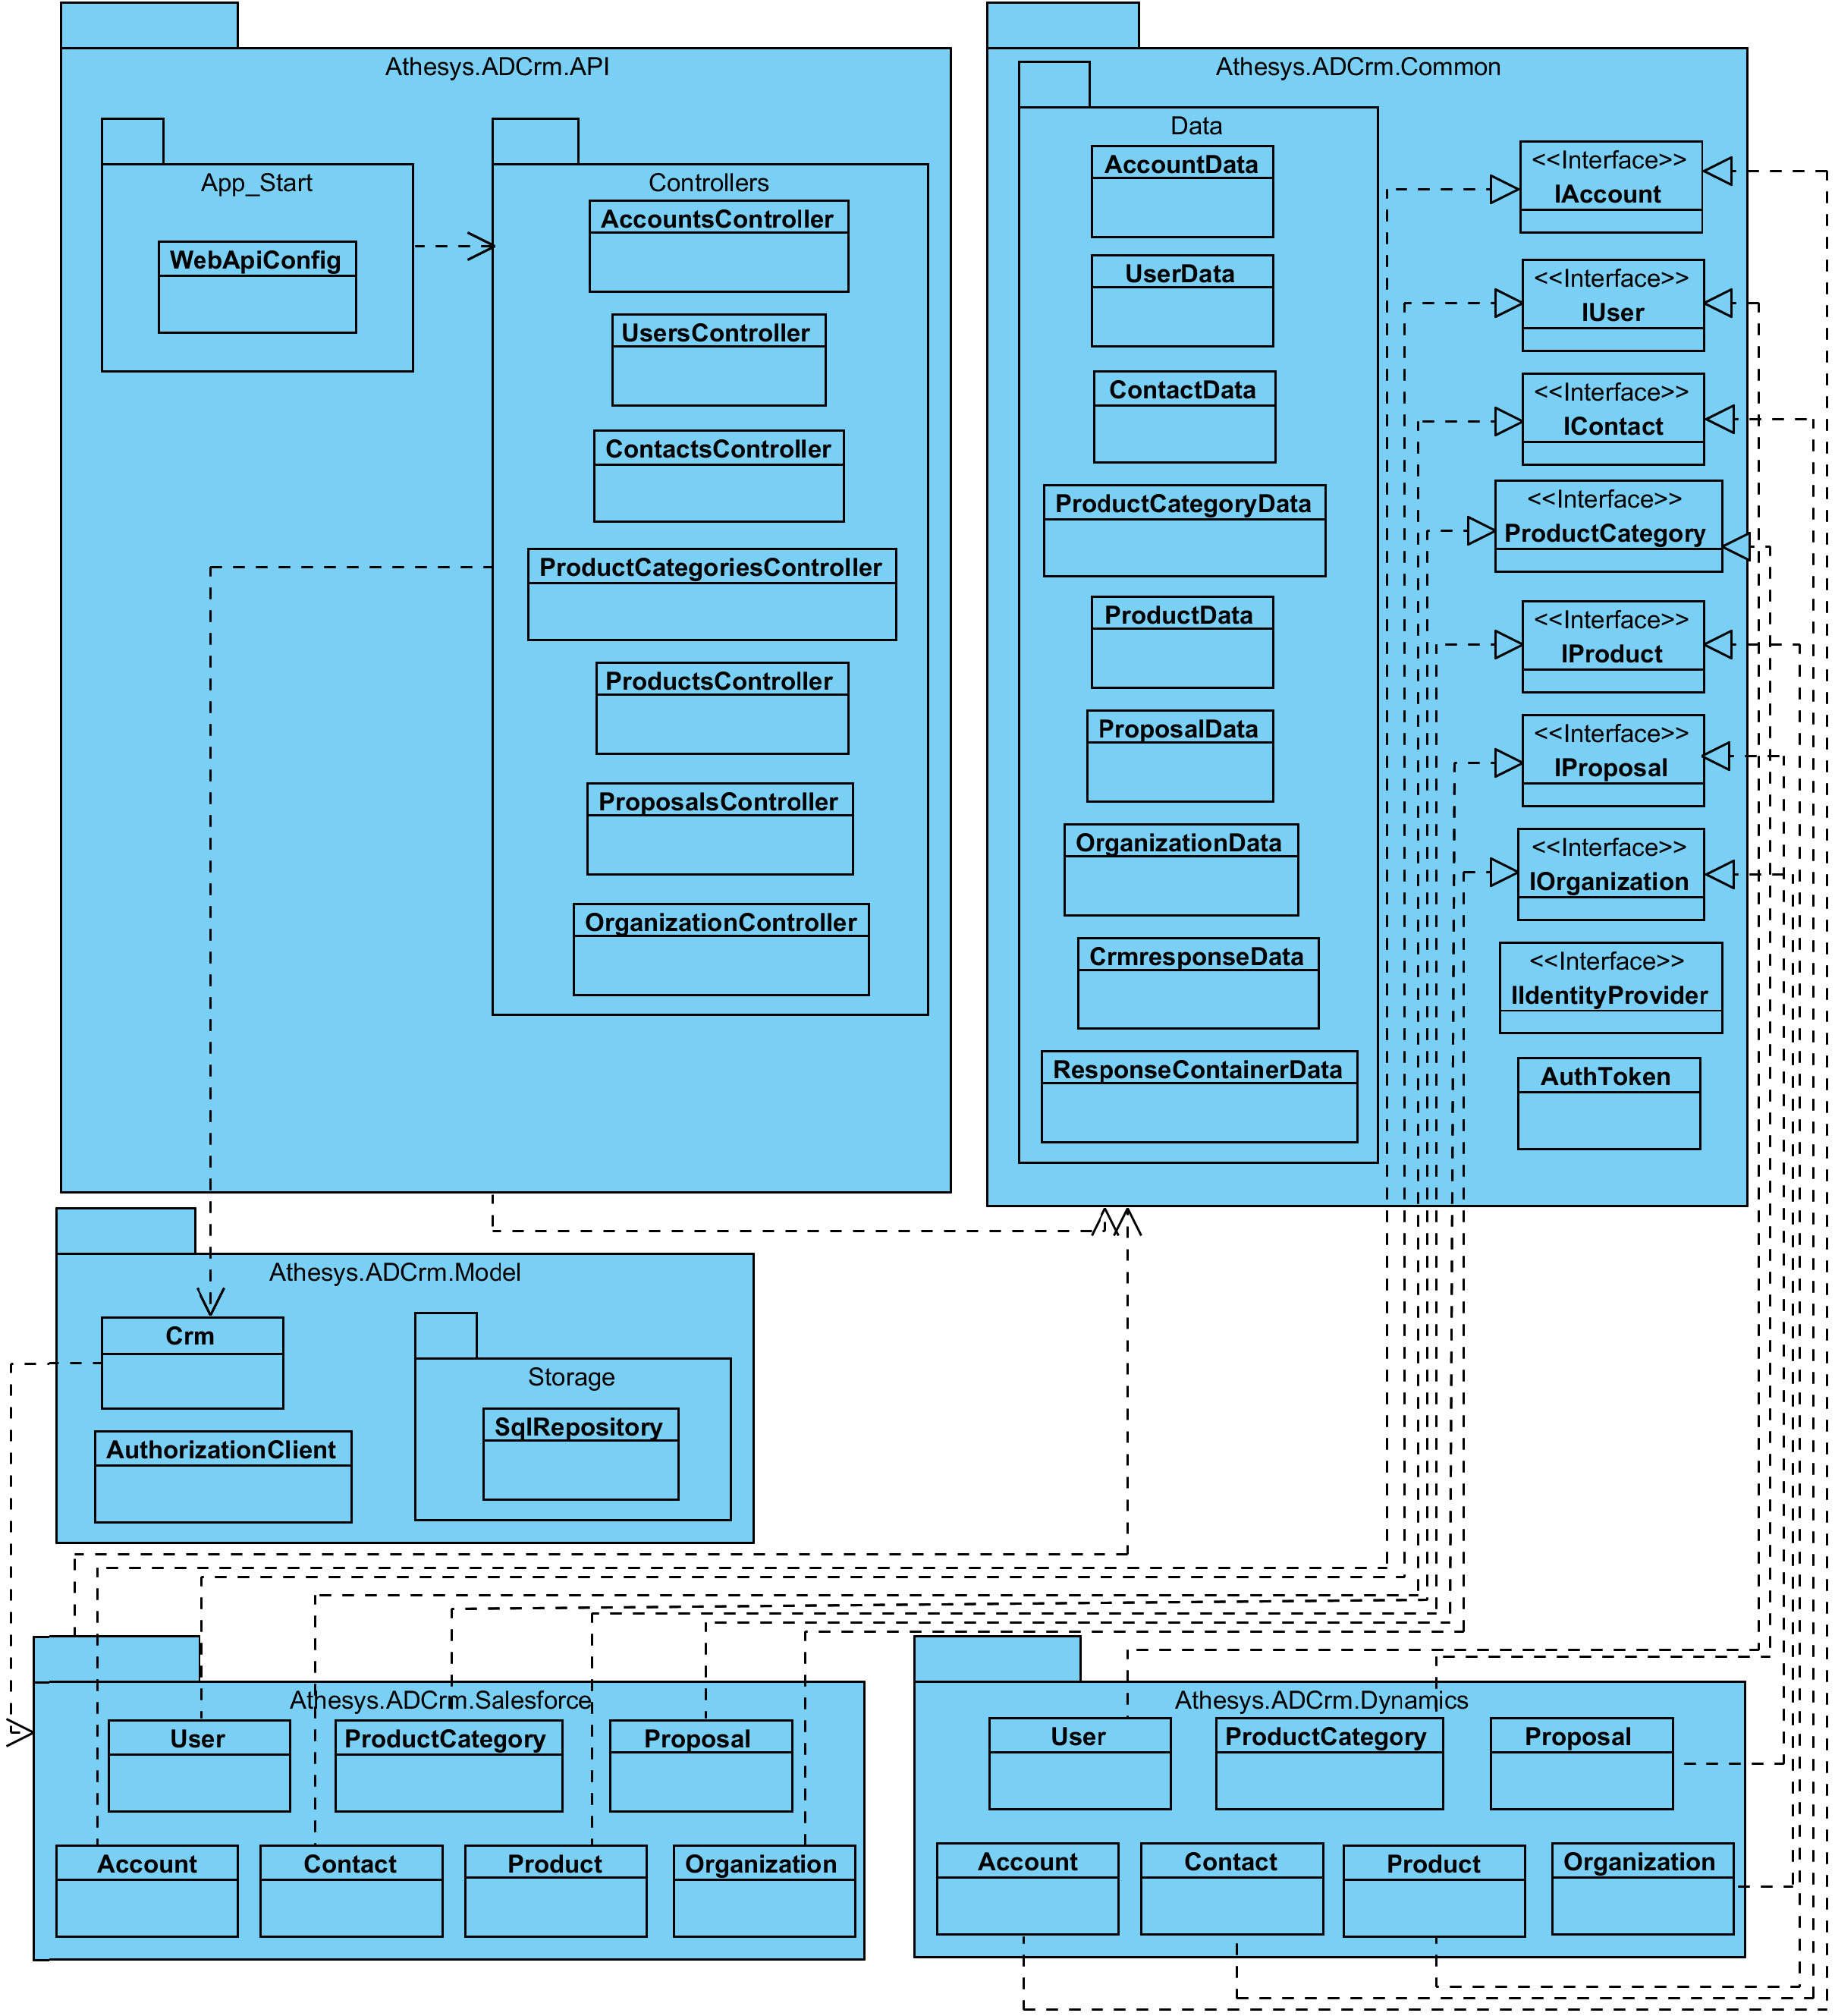
\includegraphics[width=\linewidth]{images/general2}
	\caption{Diagramma UML di ADCrm}
	\label{fig:modulesdiagram}
\end{figure}



\subsection{Athesys.ADCrm.API}

\begin{figure}[H]
	\centering
	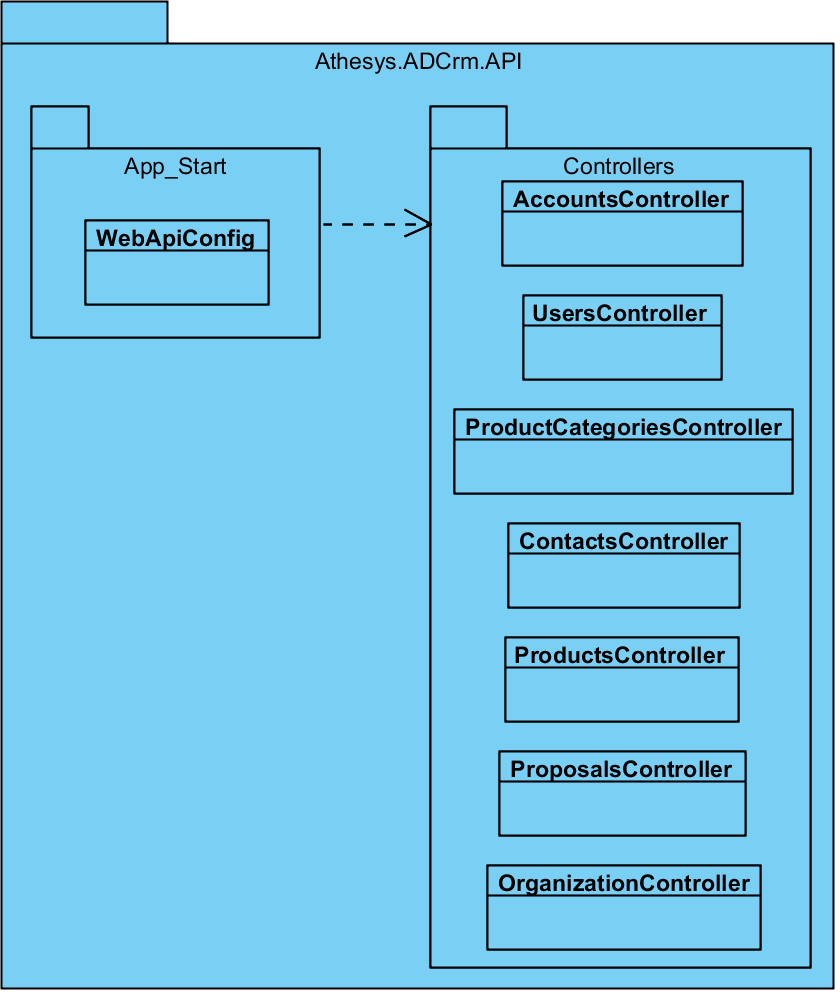
\includegraphics[width=\linewidth]{images/modules/API}
	\caption{}
	\label{fig:api}
\end{figure}

Questo \glo{package} è utilizzato per esporre le API REST all'applicazione web ADProject. In esso vengono definite le \glo{route} che è possibile chiamare e ad ognuna di esse viene associato un metodo di un particolare controller. 

\subsection{Athesys.ADCrm.API.AppStart}
Questo \glo{package} contiene la classe che si occupano di definire le \glo{route} che verranno rese disponibili dall'applicazione.

\subsection{Athesys.ADCrm.API.Controllers}

\begin{figure}[H]
	\centering
	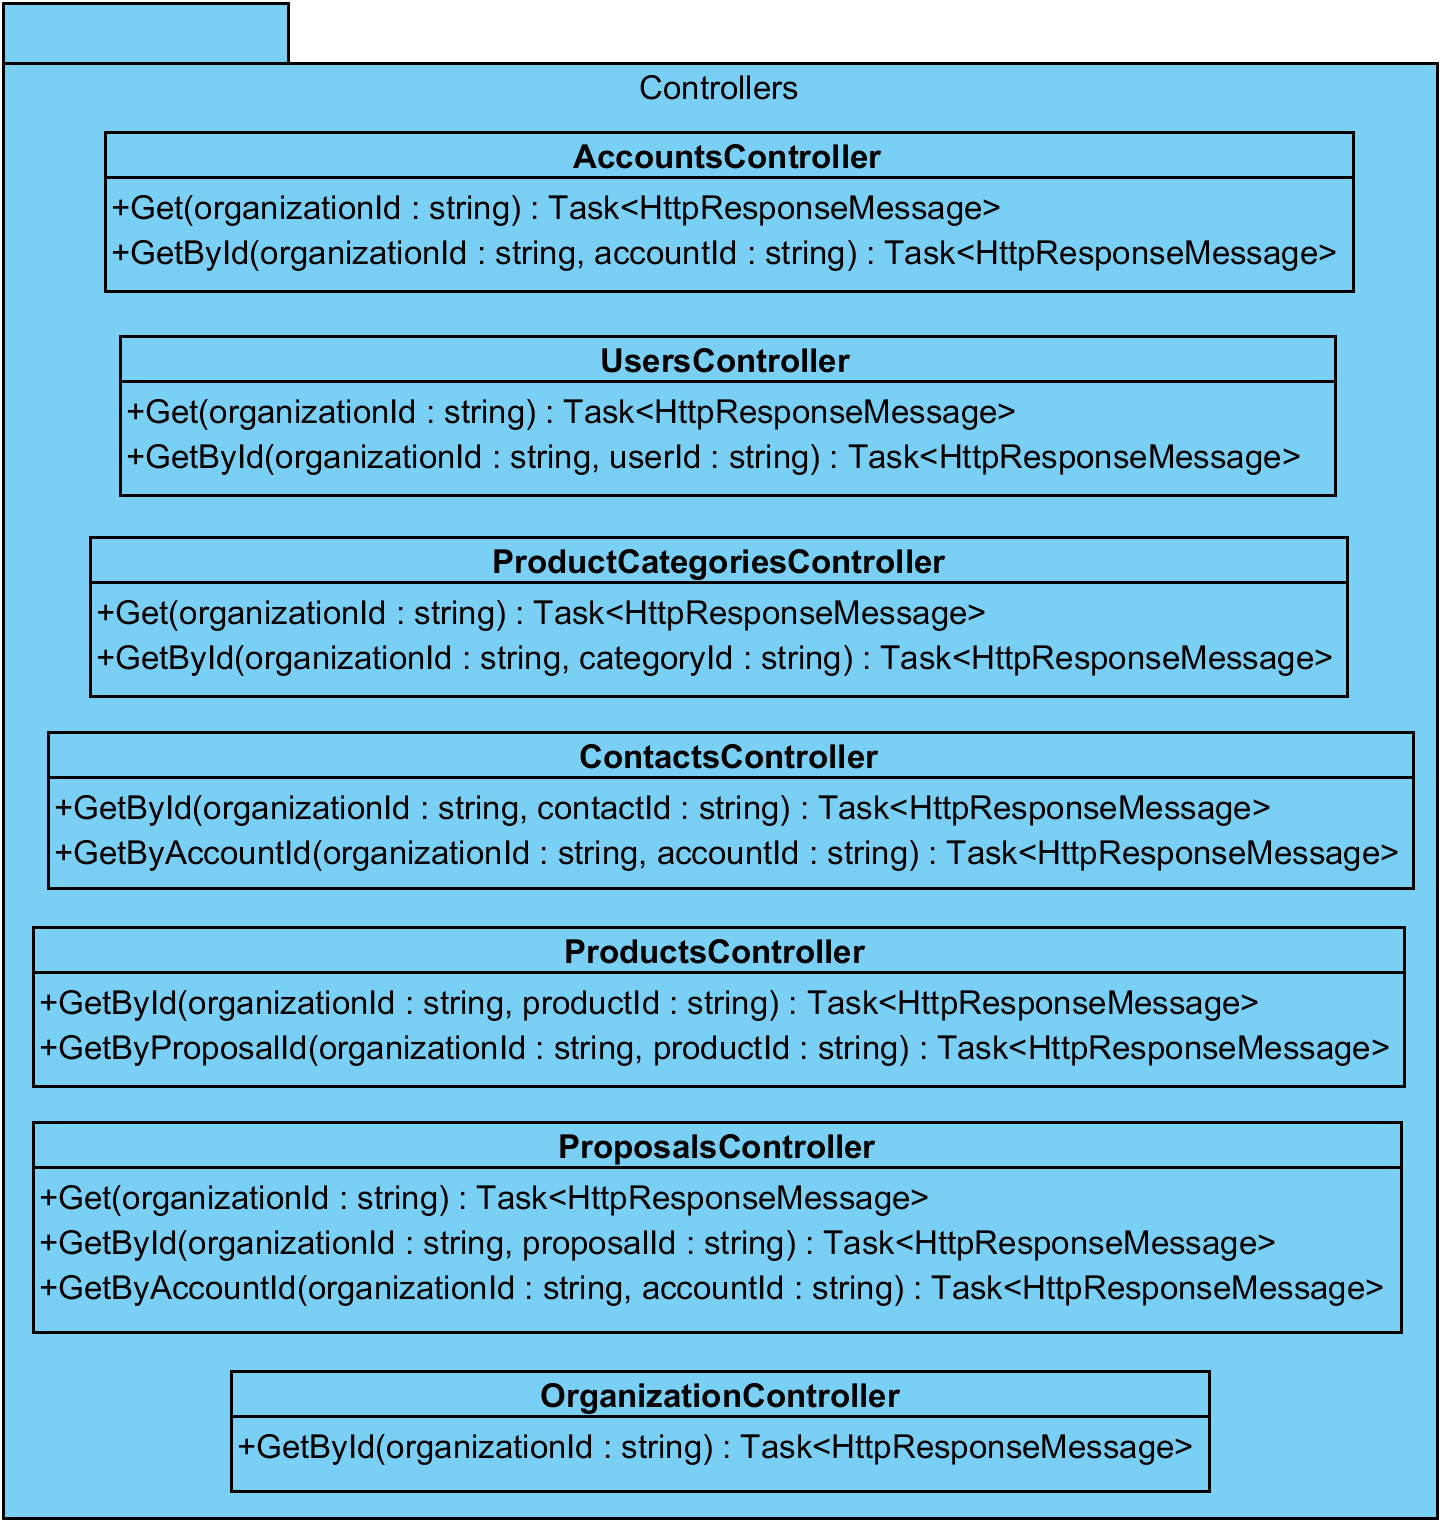
\includegraphics[width=\linewidth]{images/modules/Controllers}
	\caption{}
	\label{fig:controllers}
\end{figure}


Questo \glo{package} contiene tutte le classi controller contenenti i metodi necessari a rispondere alle richieste http effettuate alle \glo{route}.

\subsection{Athesys.ADCrm.Common}

\begin{figure}[H]
	\centering
	\includegraphics[width=\linewidth]{images/modules/common}
	\caption{}
	\label{fig:common}
\end{figure}

Questo \glo{package} contiene tutte le interfaccie e i DTO che dovranno essere implementate diversamente per ogni CRM che si vuole collegare all'applicazione. 
%TODO: da modificare la descrizione

\subsection{Athesys.ADCrm.API.Data}

\begin{figure}[H]
	\centering
	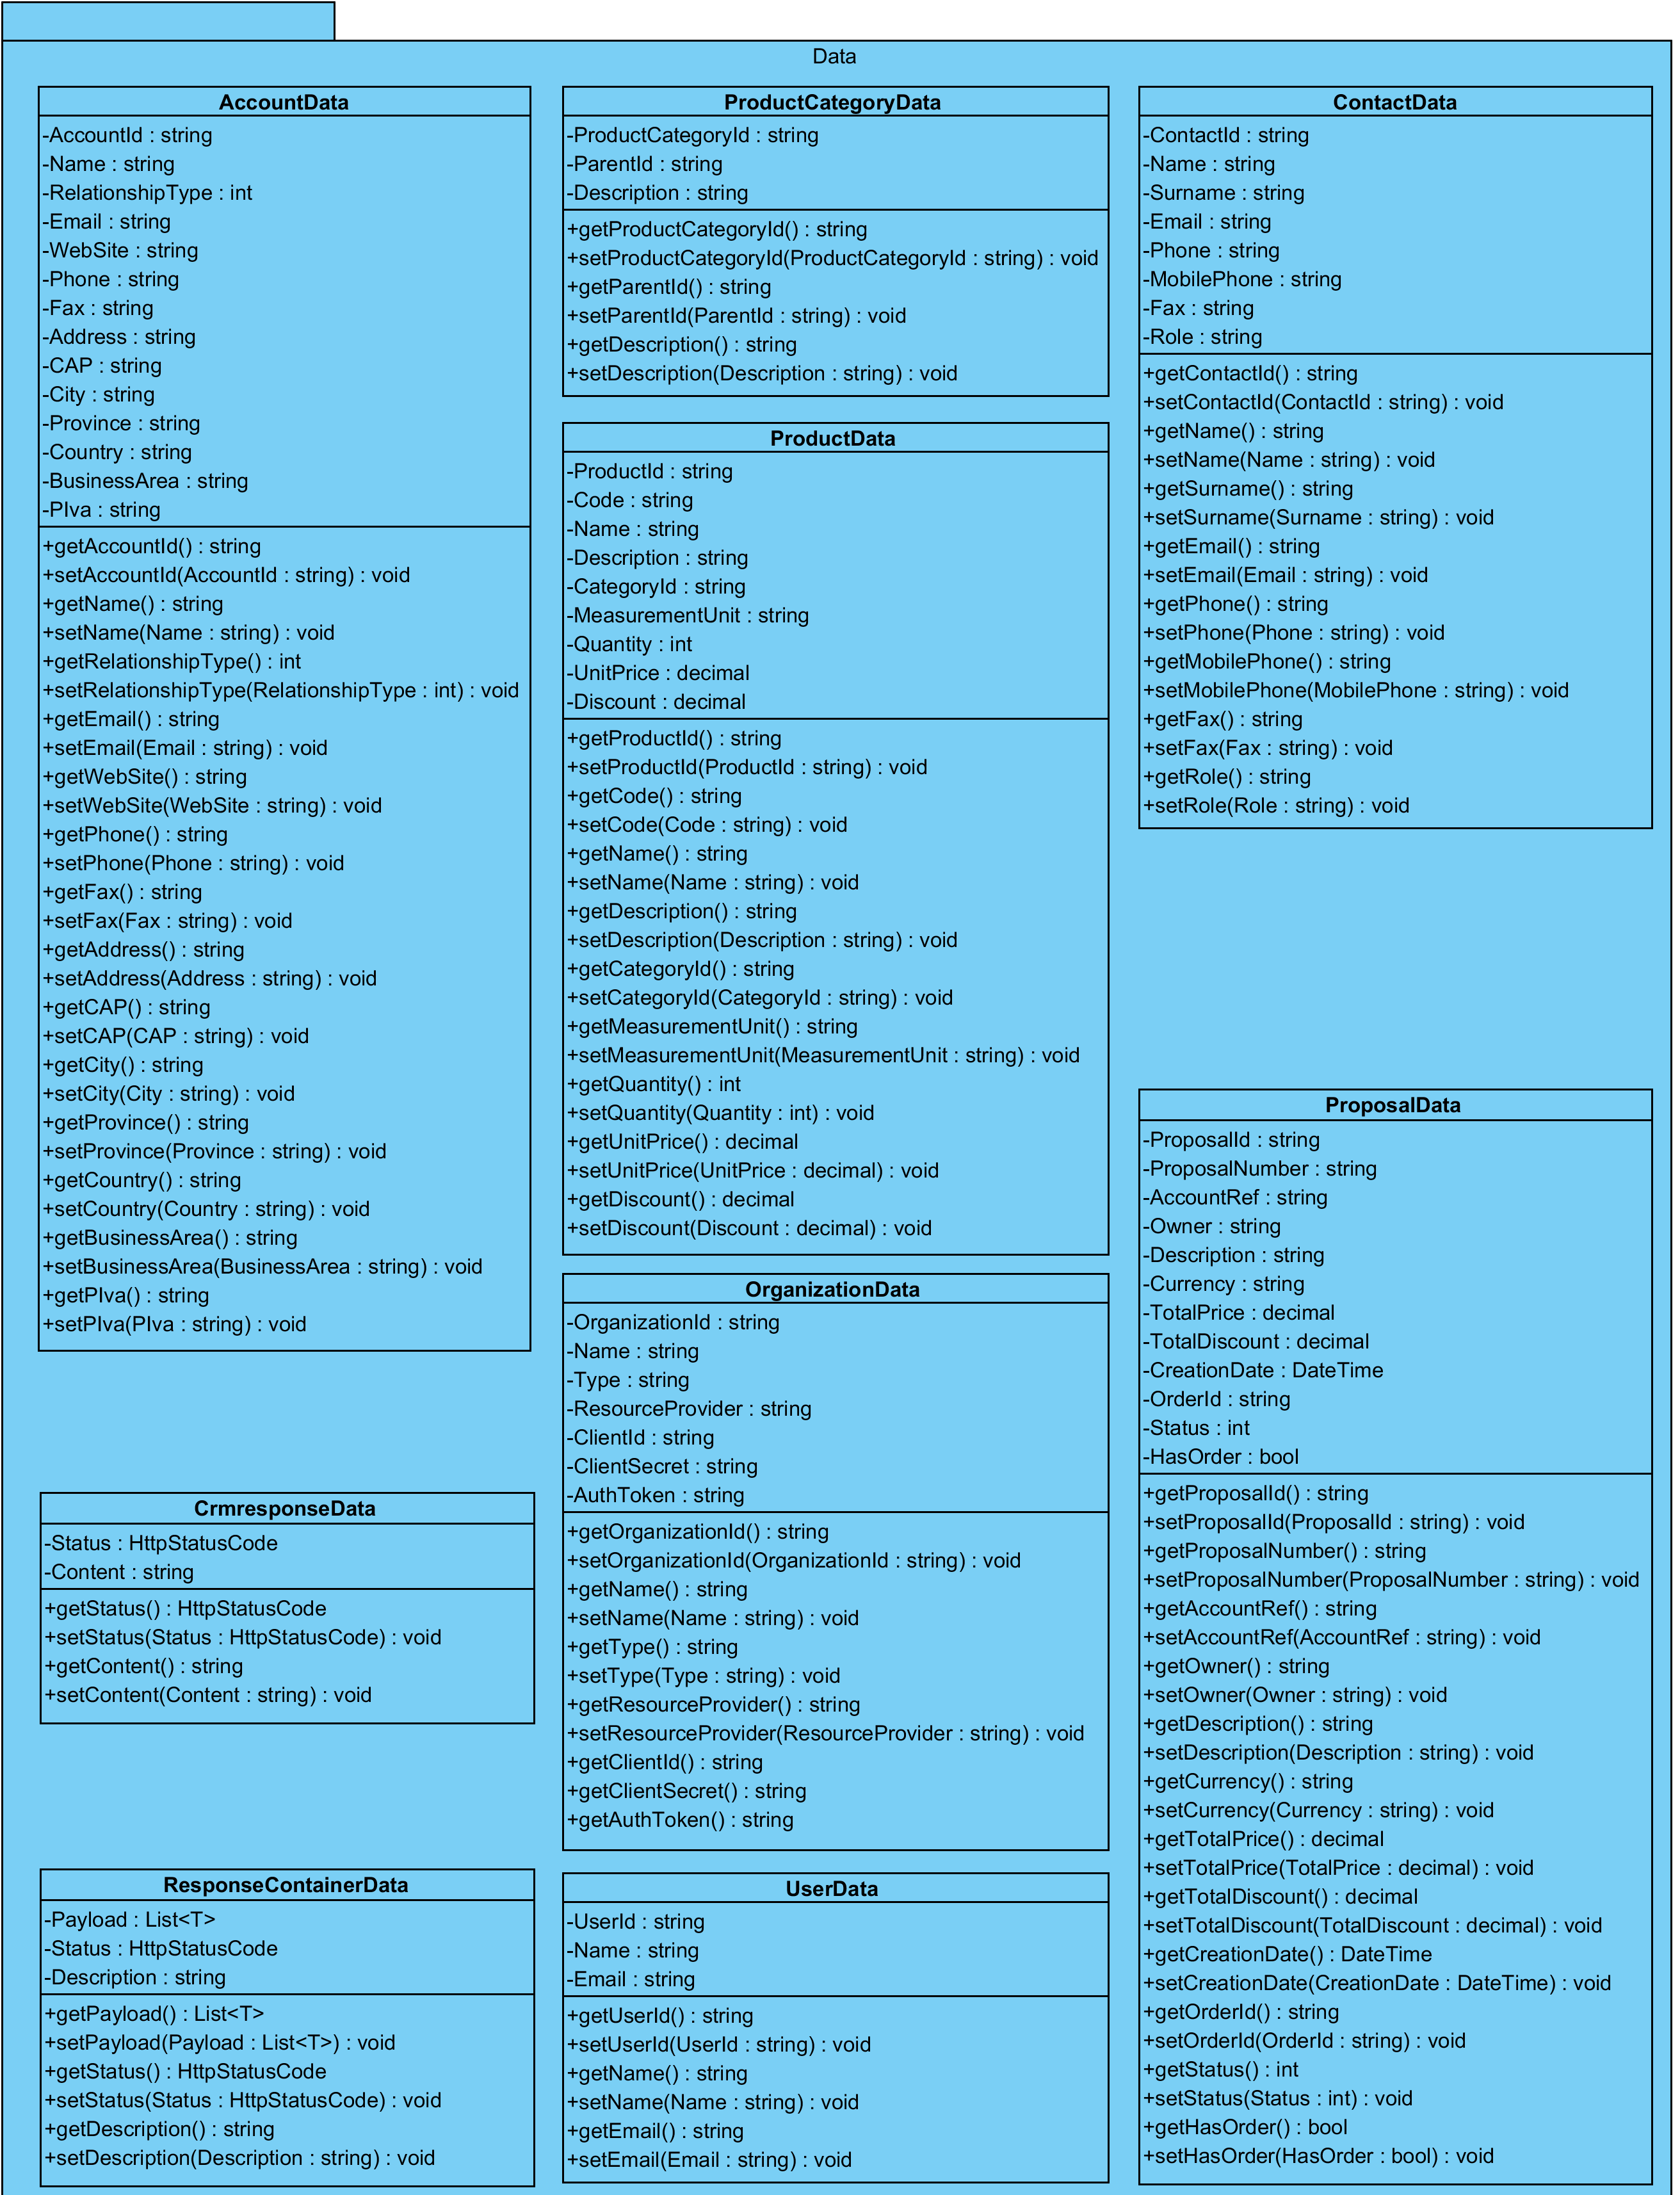
\includegraphics[width=\linewidth]{images/modules/Data}
	\caption{}
	\label{fig:data}
\end{figure}


Questo \glo{package} contiene tutti i vari DTO definiti per ogni entità di dati che si vuole restituire alle chiamate effettuate da ADProject. 

\subsection{Athesys.ADCrm.Model}
Questo package contiene tutte le classi concrete in comune tra i CRM che si vogliono collegare all'applicazione 

\subsection{Athesys.ADCrm.Salesforce}
Questo \glo{package} contiene tutte le classi che implementano le interfacce definite in Athesys.ADCrm.Common e restituiscono ai controller di Athesys.ADCrm.API i vari oggetti DTO di tipo Athesys.ADCrm.Common.Data al fine di incapsularli nella risposta HTTP.

\subsection{Athesys.ADCrm.Dynamics}
Questo \glo{package} contiene tutte le classi che implementano le interfacce definite in Athesys.ADCrm.Common e restituiscono ai controller di Athesys.ADCrm.API i vari oggetti DTO di tipo Athesys.ADCrm.Common.Data al fine di incapsularli nella risposta HTTP.